\documentclass[12pt]{article}

\usepackage{geometry}
\usepackage[russian]{babel}
\usepackage[utf8]{inputenc}
\usepackage{graphicx}
\usepackage{amsmath}
\usepackage{pgfplotstable}
\usepackage{wrapfig}
\usepackage{booktabs}
\usepackage{color, colortbl}


\newgeometry{scale = 0.85}
\selectlanguage{russian}
\setcounter{tocdepth}{5}
\renewcommand{\thesection}{\Roman{section}} 

\title{Курсовая работа по предмету "Планирование эксперимента и обработка данных"\\\textbf{Генерация второй гармоники в нелинейном кристалле}}
\date{2018-04-21}
\author{Дерека С.А., группа 642}

\begin{document}

\maketitle
\pagenumbering{gobble}
\newpage
\pagenumbering{arabic}

\vspace{0.5cm}{\parbox{17.3cm}{\small{\textbf{\centering{Аннотация}\\
				\hspace{0.6cm} В работе использовалась установка с кристаллом йодата лития. С помощью осциллографа измерили интенсивность излучения второй гармоники, сгенерированной на данном кристалле, а с помощью гониометра - угол между входным лучом и направлением синхронизма. С помощью полученных данных проверили соотношения, полученные теоретически. Также была исследована зависимость интенсивности второй гармоники от интенсивности излучения, подаваемого на кристалл, и оценён коэффициент преобразования во вторую гармонику для рассматриваемой установки.}}}}
\newpage

\section{Теоретическое введение. Генерация второй гармоники как нелинейно-оптический процесс.}

\hspace{0.5cm}
К настоящему времени созданы лазеры, позволяющие получать напряжённости электрического поля порядка $10^{8}\frac{\text{В}}{\text{см}}$. При распространении столь мощного светового пучка в среде оптические параметры среды становятся зависимыми от напряжённости поля волны. Материальное уравнение, связывающее поляризацию среды $\vec{P}$ с напряжённостью световой волны $\vec{E}$, становится нелинейным. Вынужденные колебания электрона под действием поля такой волны описываются уравнением:
\begin{equation}
x(t) = \frac{\frac{e}{m}E_0}{\omega_0^2-\omega^2}\cos{\omega t}+\frac{F''(0)}{4m\omega_0^2}\bigg[\frac{\frac{e}{m}E_0}{\omega_0^2-\omega^2}\bigg]^2+\frac{F''(0)}{4m}\bigg[\frac{\frac{e}{m}E_0}{\omega_0^2-\omega^2}\bigg]^2\frac{\cos{2\omega t}}{\omega_0^2-(2\omega)^2}
\end{equation}
\hspace{0.5cm}
Колеблющийся электрон является источником вторичных волн. Колебания диполей с удвоенной частотой $2\omega$ описываются соотношением:
\begin{equation}
X^{2\omega} = A^2\cos{2\omega}\left[t-\frac{n(\omega)}{c}z'\right]
\end{equation}
\hspace{0.5cm}
Такой диполь излучает вторичную волну частотой $2\omega$. Фаза колебаний в некоторой точке $z$ в нелинейной среде
\begin{equation}
\phi(z) = 2\omega(t-\frac{n(2\omega)}{c}z+[n(2\omega)-n(\omega)]\frac{z'}{c}),
\end{equation}
где $n(2\omega)$ - показатель преломления для частоты $2\omega$. В случае, когда
\begin{equation}
\label{synph}
\Delta n = n(2\omega) - n(\omega) = 0,
\end{equation}
фаза не зависит от расположения излучающего диполя. Тогда все вторичные волны в точке $z$ синфазны и амплитуда напряжённости $E_{0}^{(2\omega)}$ второй гармоники пропорциональна расстоянию $z$ от входной плоскости. Равенство \ref{synph} называется условием пространственной синфазности и соответствует наибольшей интенсивности второй гармоники.
\begin{wrapfigure}{r}{0.5\textwidth}
  \begin{center}
    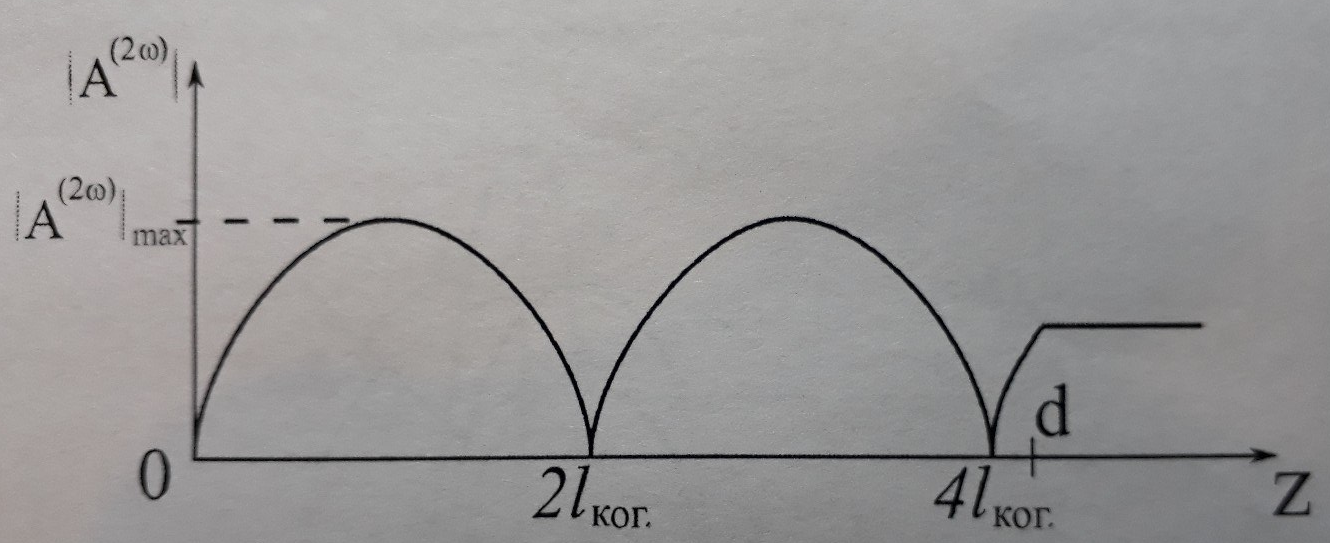
\includegraphics[width=0.48\textwidth]{pic1.png}
  \end{center}
  \caption{Зависимость амплитуды второй гармоники $|A^{2\omega}|$ от расстояния $z$.}
  \label{pic1}
\end{wrapfigure}
\hspace{0.5cm}
В общем случае амплитуда $A^{(2\omega)}$ второй гармоники определяется соотношением:
\begin{equation}
\label{inten}
A^{(2\omega)} = gA^2z\frac{\sin{k_0(\omega)\Delta nz}}{k_0(\omega)\Delta nz},
\end{equation}
т. e. амплитуда, а вместе с ней и интенсивность второй гармоники пропорциональна квадрату амплитуды и интенсивности основной волны.
\hspace{0.5cm}

На рисунке \ref{pic1} приведена зависимость амплитуды второй гармоники от координаты $z$, $d$ - точка выхода из нелинейной среды.
Максимальные значения амплитуды достигаются при условии $k_0(\omega)\Delta nz_m=\frac{\pi}{2}+\pi m$, т. е. при $z_m = l_{\text{ког}}(1+2m), m = 0,1,2,...$ Здесь $l_{\text{ког}}=\frac{\lambda}{4\Delta n}$ - длина когерентности. Если выполнено условие синфазности, то она становится бесконечно большой.
\hspace{0.5cm}

Для изотропной среды условие фазового синхронизма можно выполнить только, если частота попадает в область аномальной дисперсии. Но тогда она будет сильно поглощаться средой, и эффективной генерации второй гармоники не будет.
\hspace{0.5cm}

Можно добиться выполнения условия синхронизма, если применить в качестве нелинейной среды анизотропный одноосный кристалл. При определённом угле $\Theta_0$ между направлением распространения волны и оптической осью кристалла, выполнится условие синхронизма и основная волна является обыкновенной, а волна второй гармоники - необыкновенной. Этот угол называется углом синхронизма. Его легко рассчитать, используя зависимость показателей преломления от угла распространения луча:
\begin{equation}
n_o(\Theta) = const
\end{equation}
\begin{equation}
n_e(\Theta) = n_o\left[1+\left(\frac{n_o^2}{n_e^2}-1\right)\sin^2{\Theta}\right]^{-\frac{1}{2}}
\end{equation}
\hspace{0.5cm}
Для исследуемого кристалла йодата лития интенсивность второй гармоники зависит от интенсивности основной волны следующим образом:
\begin{equation}
\label{finaleq}
I^{(2\omega)} = k\cos^2{(\Theta-\Theta_0)}(I^{(\omega)})^2,
\end{equation}
где $k$ - коэффициент пропорциональности.

\section{Экспериментальная установка для изучения второй гармоники.}

\begin{wrapfigure}{r}{0.5\textwidth}
  \begin{center}
    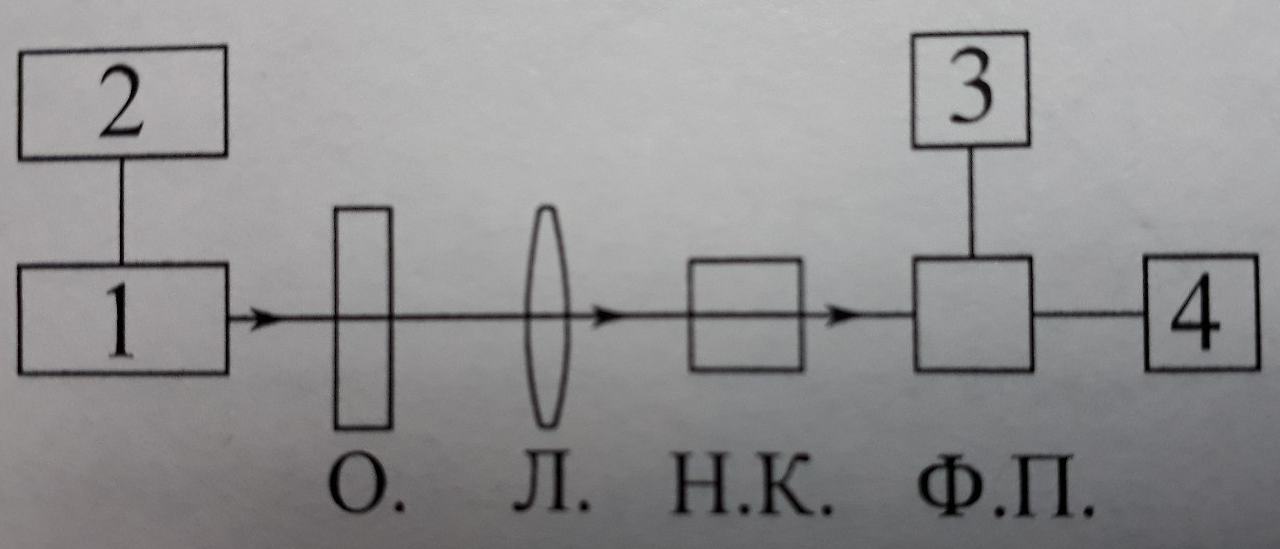
\includegraphics[width=0.48\textwidth]{pic2.png}
  \end{center}
  \caption{Схема установки для изучения второй гармоники.}
  \label{pic2}
\end{wrapfigure}
\hspace{0.5cm}
Схема установки представлена на рисунке \ref{pic2}. Здесь излучение лазера 1, пройдя ослабитель О. и линзу-корректор Л., попадает в нелинейный кристалл Н.К., где частота его удваивается. Излучение удвоенной частоты далее попадает в фотоприёмник Ф.П. и регистрируется осциллографом 4. 2 и 3 - блоки питания.

\textbf{1.}\textbf{Лазер.} Используется твердотельный лазер ЛКС-ДЛТ-112ОТ, который работает в режиме модуляции добротности на двух длинах волн одновременно: $\lambda_1$ = 1064 нм, $\lambda_2$ = 532 нм. Ослабитель служет для изменения интенсивности излучения, падающего на нелинейный кристалл. Он имеет четыре окна, обеспечивающие различное ослабление интенсивности. Линза-корректор уменьшает расходимость пучка, выходящего из лазера.

\textbf{2.}\textbf{Нелинейный кристалл.} Кристалл $LiIO_3$ крепится к столику гониометра при помощи магнитов. Излучение лазера попадает в центр входного окна кристалла и отражается в обратном направлении. Кристалл выпилен таким образом, что угол $\Theta_0=32^{\circ}$ между нормалью к поверхности и оптической осью есть угол синхронизма.

\textbf{3.}\textbf{Гониометр.} Используется модель Г5М. Его ошибка измерения угла составляет $\pm 5''$. С помощью гониометра определяется ориентация кристалла относительно направления распространения излучения лазера.

\textbf{4.}\textbf{Фотоприёмник.} Интенсивность излучения, выходящего из кристалла, регистрируется фотоприёмником, подключённым к осциллографу. Для измерения отдельных интенсивностей основной волны и второй гармоники используются светофильтры, которые размещаются на фотоприёмнике.

\section{Программное обеспечение для обработки и визуализации данных.}

\hspace{0.5cm}
В ходе данной работы были использованы следующие инструменты анализа данных:
\begin{itemize}
\item[•] LibreOffice Calc - внесение данных в таблицы и их предобработка.
\item[•] Pandas - работа с данными в формате .csv.
\item[•] Matplotlib - для визуализации данных на графиках.
\item[•] Scipy - статистические методы ( например, вычисление корреляции ).
\item[•] Statsmodels - статистические методы ( например, МНК ).
\end{itemize}

\section{Исследование зависимости интенсивности линии второй гармоники $\lambda$ = 532 нм от интенсивности возбуждющей линии $\lambda$ = 1064 нм.}

\hspace{0.5cm}
В данном опыте исследуемый кристалл при помощи гониометра располагается так, чтобы интенсивность второй гармоники была максимальна ( достигается синхронизм ). При помощи осциллографа измеряются интенсивности возбуждающей линии и второй гармоники. Согласно соотношению \ref{inten}, связь между этими величинами выражается следующим образом:
\begin{equation}
\label{hyp1}
I^{(532)} = \alpha{I^{(1064)}}^2,
\end{equation}
где $\alpha$ - коэффициент пропорциональности. Цель эксперимента состоит в проверке этого соотношения.

\begin{table}[h!]
\begin{center}
\caption{Показания осциллографа для интенсивностей основной волны и второй гармоники}
\label{tab1}
\pgfkeys{/pgf/number format/.cd,fixed,fixed zerofill,precision=1}
\pgfplotstabletypeset[
multicolumn names,
col sep = comma,
columns/first/.style={column name = {$I^{(1064)},2\text{В}$} },
columns/first2/.style={column name = {${I^{(1064)}}^2,(2\text{В})^2$} },
columns/second/.style={column name = {$I^{532},50\text{мВ}$} },
columns/sigma/.style={column name = {$\sigma_I, 2\text{В}/50\text{мВ}$} },
columns/sigma2/.style={column name = {$\sigma_{{I^{(1064)}}^2}, (2\text{В})^2$} },
every head row/.style={before row=\toprule, after row=\midrule },
every even row/.style={before row={\rowcolor[gray]{0.9}}},
every last row/.style={after row=\midrule },
]{1.csv}
\end{center}
\end{table}

В таблице \ref{tab1} приведены результаты измерения интенсивностей $I^{(532)}$ и $I^{(1064)}$ при помощи осциллографа. Согласно предположению \ref{hyp1}, между величинами $I^{(532)}$ и ${I^{(1064)}}^2$ должна существовать линейная связь. Вычислим для них коэффициент корреляции Пирсона:
\begin{equation}
r_{I^{(532)}{I^{(1064)}}^2} = 0.996
\end{equation}
Полученное значение близко к единице, что позволяет говорить о том, что данные величины линейно коррелированы.

Применим метод наименьших квадратов для определения коэффициента $\alpha$. Приняв свободный член модели равным нулю, получим:
\begin{equation}
\alpha = 0.192\pm 0.009
\end{equation}

На рисунке \ref{pic3} представлен график зависимости интенсивности линии второй гармоники от квадрата интенсивности возбуждющей линии. Как можно видеть, данная зависимость является линейной. Таким образом, в данном эксперименте установлена справедливость соотношения \ref{hyp1}.

\begin{figure}[h!]
  \begin{center}
    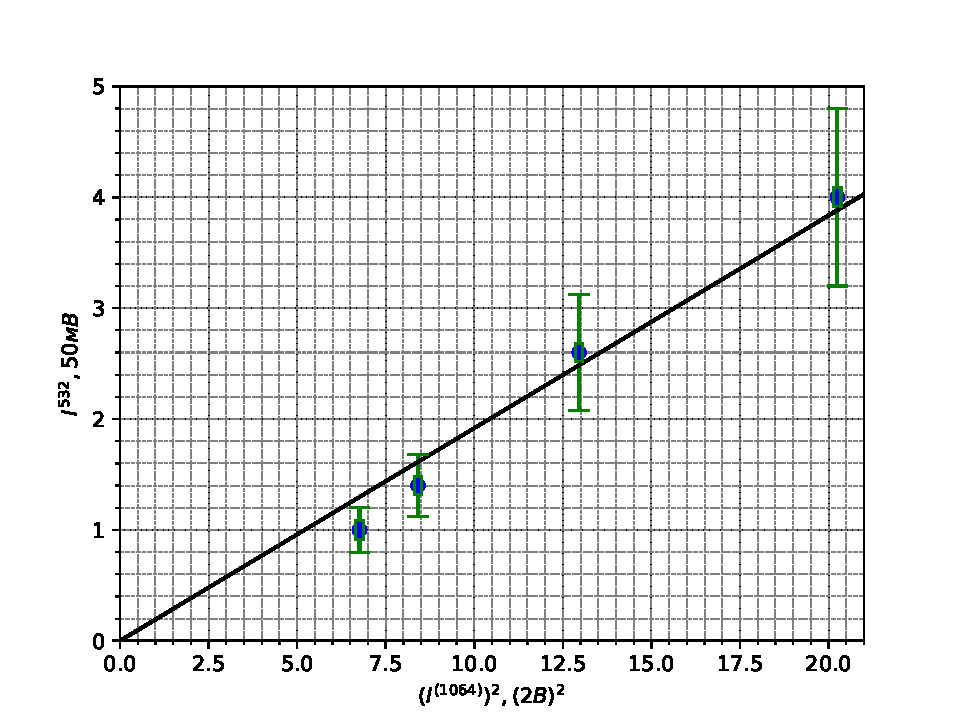
\includegraphics[width=\textwidth]{pic3.pdf}
  \end{center}
  \caption{Зависимость интенсивности второй гармоники от квадрата интенсивности возбуждющей волны}
  \label{pic3}
\end{figure}

\section{Исследование зависимости интенсивности второй гармоники $I^{(532)}$ от угла $\Delta \Theta = \Theta - \Theta_0$ между направлением распространения основной волны $\lambda$ = 1064 нм и направлением синхронизма.}

\hspace{0.5cm}
В данном эксперименте при помощи гониометра изменяется угол $\Delta \Theta = \Theta - \Theta_0$, а на осциллографе регистрируется интенсивность второй гармоники. Согласно соотношению \ref{finaleq}, при фиксированной интенсивности лазерного излучения связь между интенсивностью второй гармоники и отклонением от направления синхронизма представима следующим образом:
\begin{equation}
\label{hyp2}
I^{(532)} = \beta \cos^2{(\Delta \Theta)},
\end{equation}
где $\beta$ - коэффициент пропорциональности. Задачей данного эксперимента является проверка справедливости соотношения \ref{hyp2}.

В таблице \ref{tab2} приведены показания осциллографа и гониометра.

\begin{table}[h!]
\begin{center}
\caption{Исследование зависимости интенсивности второй гармоники $I^{(532)}$ от угла $\Delta \Theta$}
\label{tab2}
\pgfkeys{/pgf/number format/.cd,fixed,fixed zerofill,precision=5}
\pgfplotstabletypeset[
columns = {gon, delta, delta2e7, sigma2e7, sigma, I, sigmai},
multicolumn names,
col sep = comma,
columns/gon/.style={column name = {$\Theta,\text{рад}$}},
columns/delta/.style={column name = {$\Delta \Theta,\text{рад}$}, sci},
columns/delta2e7/.style={column name = {$\Delta \Theta ^2,10^{-7}\text{рад}^2$}, precision=4, sci},
columns/sigma2e7/.style={column name = {$\sigma_{\Delta \Theta ^2},10^{-7}\text{рад}^2$}, precision=4, sci},
columns/sigma/.style={column name = {$\sigma_{\Delta \Theta},\text{рад}$}, sci},
columns/I/.style={column name = {$I^{(532)}, 50\text{мВ}$}, precision=1 },
columns/sigmai/.style={column name = {$\sigma_{I^{(532)}}, 50\text{мВ}$}, precision=1},
every head row/.style={before row=\midrule, after row=\midrule},
every even row/.style={before row={\rowcolor[gray]{0.9}}},
every last row/.style={after row=\midrule},
]{2.csv}
\end{center}
\end{table}

С учётом малости угла $\Delta \Theta$ соотношение \ref{hyp2} принимает вид:
\begin{equation}
\label{hyp2sub}
I^{(532)} = A + B\Delta \Theta ^2,
\end{equation}
т. е. между величинами $I^{(532)}$ и $\Delta \Theta ^2$ должна существовать линейная связь.

Рассчитаем коэффициент корреляции Пирсона для этих величин:
\begin{equation}
r_{I^{(532)}\Delta \Theta ^2} = -0.993
\end{equation}

Полученное значение близко по модулю к единице. Исследуемые величины линейно коррелированы. Определим коэффициенты в соотношении \ref{hyp2sub} методом наименьших квадратов:
\begin{equation}
A = 3.53\pm 0.05,\ B = -0.041\pm 0.001
\end{equation}

\begin{figure}[h!]
  \begin{center}
    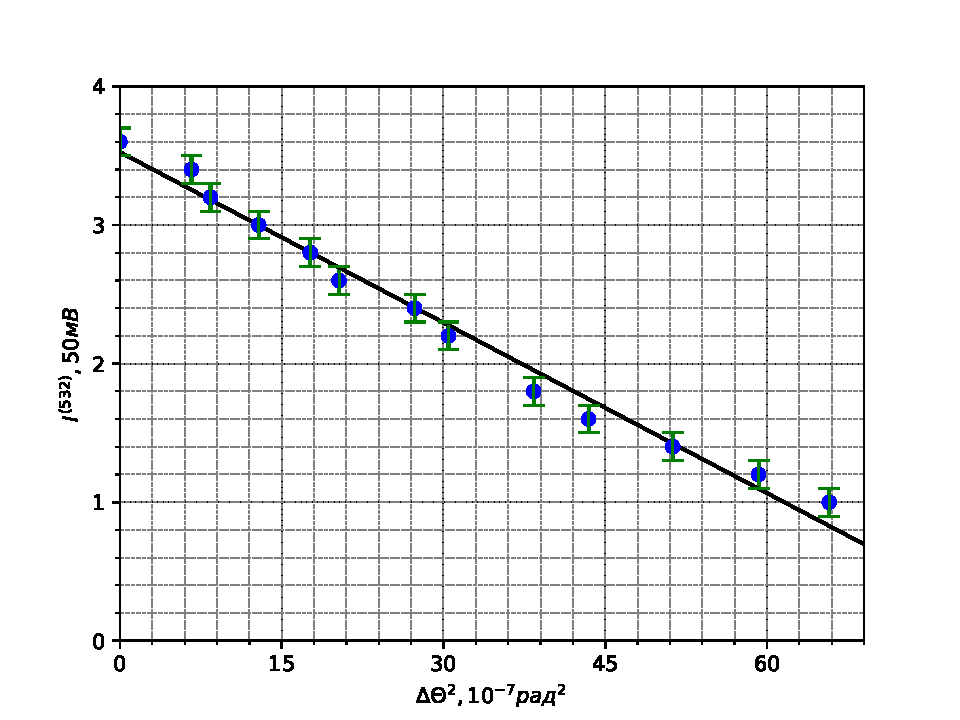
\includegraphics[width=\textwidth]{pic4.pdf}
  \end{center}
  \caption{Зависимость интенсивности второй гармоники от квадрата отклонения от направления синхронизма}
  \label{pic4}
\end{figure}

На рисунке \ref{pic4} изображена зависимость $I^{(532)}=f(\Delta \Theta ^2)$. Можно видеть, что данная зависимость близка к линейной. Итак, найденная экспериментально связь между исследуемыми величинами находится в соответствии с теоретически обнаруженной зависимостью.

\section{Оценка коэффициента преобразования во вторую гармонику для исследуемой установки.}

\hspace{0.5cm}
Пусть $\Delta I(\omega)$ - разница интенсивностей возбуждающей линии при отсутствии второй гармоники и когда её интенсивность максимальна. Тогда коэффициент преобразования во вторую гармонику установки определяется следующим образом:
\begin{equation}
K = \frac{\Delta I(\omega)}{I(\omega)},
\end{equation}
где $I(\omega)$ - интенсивность возбуждающей линии при отсутствии второй гармоники.

Оценим эту величину: $\Delta I^{(1064)} = (0.20\pm 0.01)\text{В},\ I^{(1064)} = (9.0\pm 0.2)\text{В}$. Тогда для искомой величины имеем:
\begin{equation}
K = 0.020 \pm 0.001
\end{equation}

Можно видеть, что лишь незначительная часть энергии возбуждающей линии преобразуется во вторую гармонику.

\section{Результаты работы.}

\hspace{0.5cm}
В ходе работы было установлено следующее:
\begin{itemize}
\item[•] Интенсивность второй гармоники зависит квадатично от интенсивности основной волны и при малых отклонениях от направления синхронизма пропорциональна квадрату отклонения.
\item[•] Определён коэффициент преобразования во вторую гармонику данной установки.
\end{itemize}

\bibliographystyle{ieeetr}

\end{document}\grid
